% первая часть

\section{Описание предметной области}
В ходе выполнения проекта, главным образом, решается задача преобразования двумерных изображений в трехмерные(GIF) на мобильных устройствах.

В последние годы заметное место в области преобразования и фильтрации изображений занимает задача преобразования двумерных изображений в трехмерные. На сегодняшний день в мире для этого разработаны различные методики, которые позволяют автоматически создавать так называемые «карты глубины» для двумерных изображений, основываясь на свойствах этого изображение и на некоторых предположениях о характере сцены. 

\subsection{Выбор архитектуры мобильного приложения}
В ходе выполнения работы были рассмотрены различные варианты для создания мобильных приложений, предназначенных для преобразования 2D изображений в 3D вид. При этом рассмотрении учитывалось, что результирующие мобильные приложения должны создаваться под операционные системы Android, а также то, что один из основных результатов работы приложения с точки зрения конечного пользователя – это возможность публикации созданного 3D-изображения в виде анимированного gif-файла в одном или нескольких аккаунтов в социальных сетях пользователя. Соответственно, можно исходить из предположения о том, что для функционирования приложения в любом случае необходим доступ к сети интернет. Максимальная унификация различных составных частей приложения между собой хотя бы на уровне исходных кодов вне зависимости от целевой платформы (Android или iOS) является дополнительным преимуществом при рассмотрении различных вариантов создания мобильных приложений.

Один из наиболее простых с технической точки зрения вариантов реализации решения, позволяющего преобразовывать 2D файлы в 3D вид, является решение, основанное на создании веб-сервиса, который предоставляет минимально необходимый пользовательский интерфейс для загрузки желаемого файла на сервер, преобразования файла на сервере и, как результат, возможность скачать получившийся файл на устройство пользователя и поделиться этим файлом в социальных сетях. При простоте архитектуры у этого решения есть один существенных недостаток – как правило, такие решения менее удобны и функциональны, чем нативные (native) мобильные приложения, разработанные специально под целевую платформу, на которой они будут функционировать.

Рассмотрим два варианта создания нативных мобильных приложений:

\begin{enumerate}
	\item Использовать наиболее популярные средства разработки и языки программирования для каждой из необходимых мобильных платформ. Создать нативное мобильное приложение, реализующее весь необходимый пользовательский интерфейс, набор сервисных функций. Портировать алгоритм преобразования графического файла из 2D в 3D для локального исполнения на мобильном устройстве. Все необходимые преобразования выполнять локально, на мобильном устройстве. Полученный результат преобразования (анимированный gif) загружать в интернет (социальные сети) по мере его готовности на мобильном устройстве.
	
	\item Использовать наиболее популярные средства разработки и языки программирования для каждой из необходимых мобильных платформ для создания нативных мобильных приложений только для реализации пользовательского интерфейса и набора сервисных функций. Алгоритм преобразования графического файла из 2D в 3D реализуется в виде серверного модуля, соответственно для преобразования выбранного файла и предварительного просмотра полученных результатов необходимо загрузить этот выбранный файл на сервер. Загрузить полученный результат с сервера и поделиться этим результатом в социальных сетях.
\end{enumerate}

Для варианта №1 для операционной системы Android необходимо:

С использованием Android Studio на языке программирования Java реализовать необходимый пользовательский интерфейс, а также весь необходимый набор сервисных функций. Необходимо адаптировать реализацию алгоритма преобразования графического файла из 2D в 3D для использования под управлением операционной системы Android (реализация на С++). Далее, с использованием механизма The Android Native Development Kit (NDK) необходимо обеспечить вызов кода, написанного на языке С++ из «классического» Android-приложения. 

Для реализации варианта №2 необходимо:

С использованием Android Studio на языке программирования Java необходимо создать нативное мобильное приложение для реализации пользовательского интерфейса и набора сервисных функций. Эта задача, в целом, является типовой и принципиальных сложностей не вызывает. Алгоритм преобразования графического файла из 2D в 3D следует реализовать в виде серверного модуля, например, для использования под управлением операционной системы Ubuntu. Это обусловлено тем, что Unix-подобные операционные системы имеют существенно более широкое распространение в Web-серверном окружении, чем Windows-сервера.

На основе проведенного исследования моно сделать следующий вывод. С точки зрения скорости, легкости и качества реализации наиболее перспективными являются вариант №2. 

Очевидным недостатком подобного решения является существенная его зависимость от скорости и надежности мобильного интернета, а также от доступности конечному пользователю оплаченного трафика. Для обхода этих ограничений предполагается исследовать возможность создания для пользователей ОС Android «самодостаточного» мобильного приложения (вариант №1), которое все необходимые действия, связанные с преобразованием файлов производит непосредственно на мобильном устройстве.


\section{Проектирование структуры приложения}

Одна из важнейших задач в ходе создания мобильного приложения, преобразовывающего 2D снимки в объемные (3D) - разработка удобного и интуитивно-понятного пользовательского интерфейса. UI/UX (user Interface, user experience) составляющая, она же пользовательский интерфейс и пользовательский опыт, является более чем просто значимым элементом современного мобильного приложения. Удобство расположения элементов управления и приятное визуальное оформление напрямую влияют на настроение пользователя при использовании продукты. Именно некачественный UI/UX-дизайн отпугивает людей от использования многих приложений в пользу их более достойных альтернатив.

На главный экран камеры (рисунок~\ref{fig:Artboard}) выведены следующие функции:

\begin{itemize}
	\item Спуск затвора;
	\item Выбор фото из галереи;
	\item Смена камеры;
	\item Управление вспышкой;
	\item Переход к настройкам и справке.
\end{itemize}

\begin{figure}[H]
	\centering
	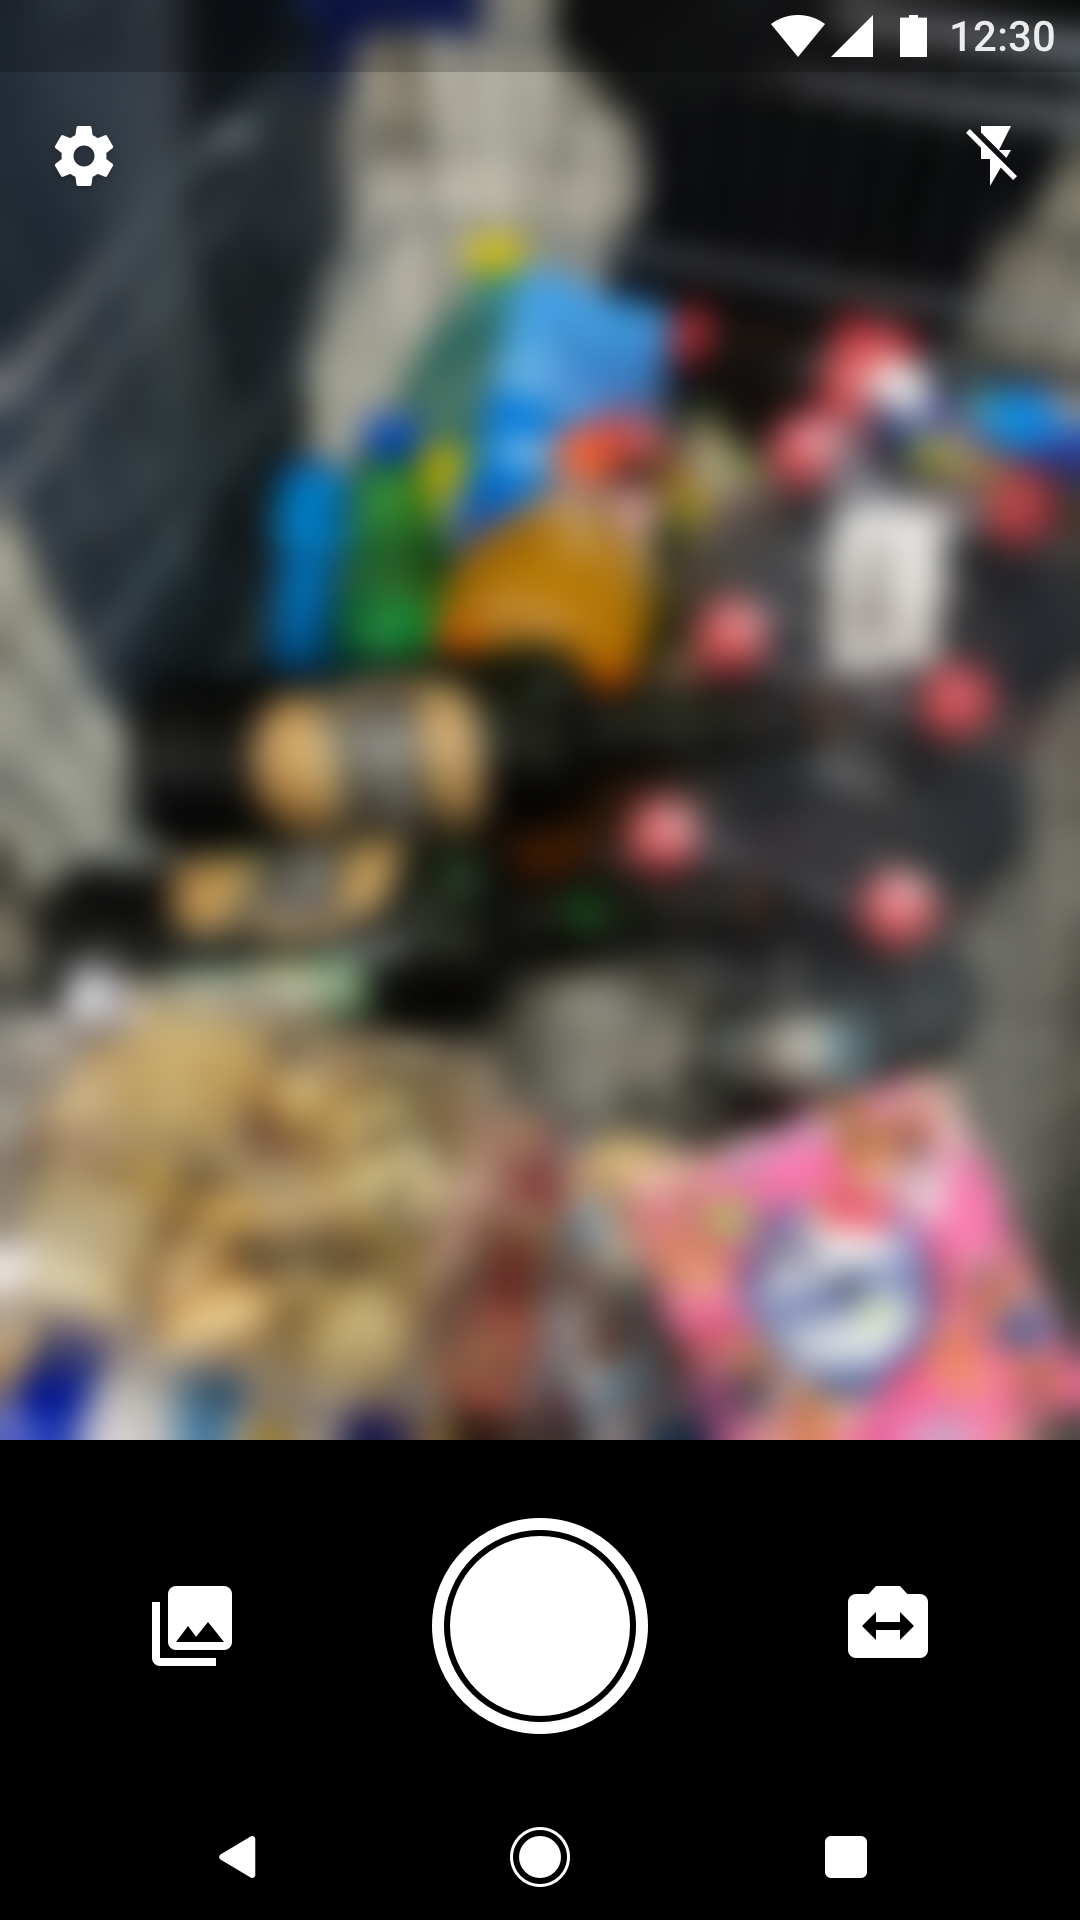
\includegraphics[width=0.4\linewidth]{pics/Artboard}
	\caption{Окно с камерой}
	\label{fig:Artboard}
\end{figure}

На экране с обработанной фотографией по нажатии кнопки «Далее» появляется bottom sheet (рисунок~\ref{fig:Artboard2}), включающий в себя быстрые функции шеринга и сохранения полученного фото в галерею.

\begin{figure}[H]
	\centering
	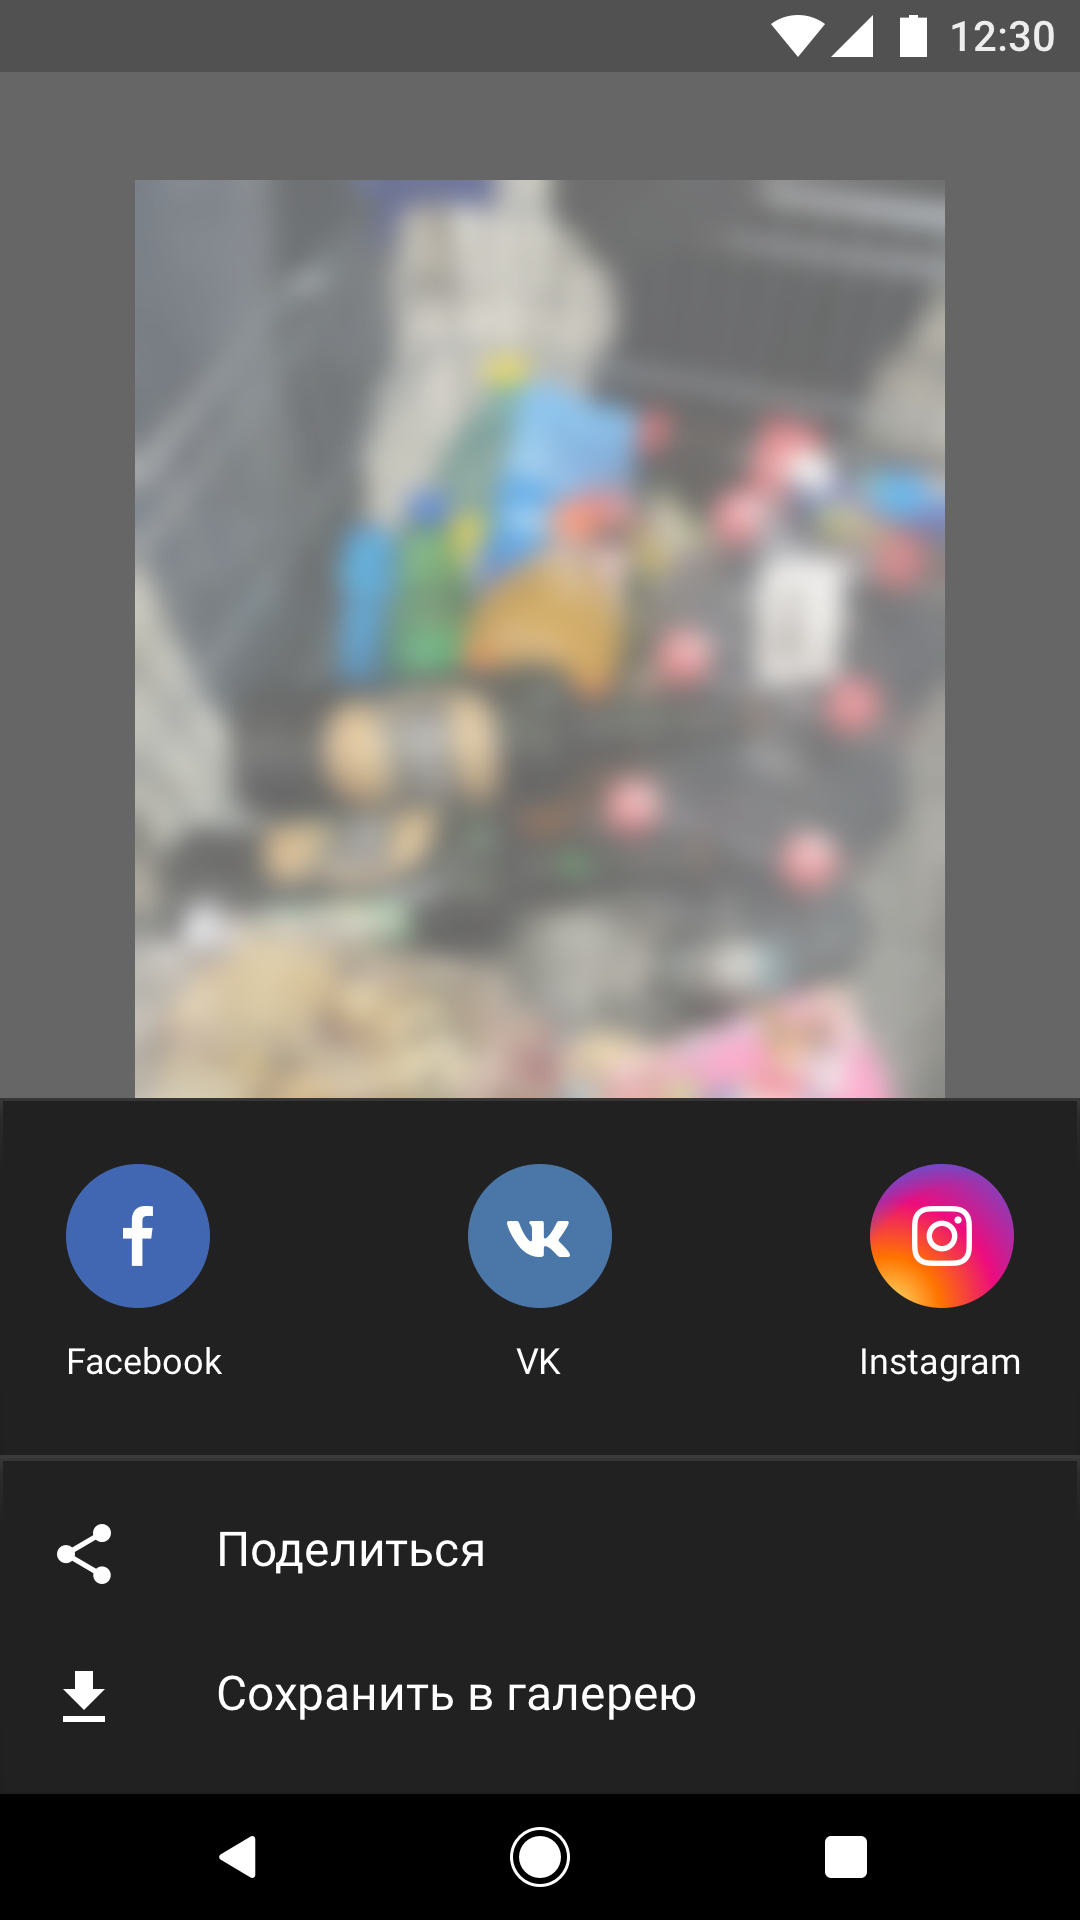
\includegraphics[width=0.4\linewidth]{pics/Artboard2}
	\caption{Окно с просмотром фото}
	\label{fig:Artboard2}
\end{figure}

При создании пользовательского интерфейса приложения были проанализированы современные, с аналогичным функционалом мобильные приложения в целом. Был сделан акцент на необходимости создания современного, функционального и не перегруженного пользовательского интерфейса. В результате проведенного анализа был создан пользовательский интерфейс мобильного приложения для преобразования 2D фотографий в 3D вид.

\subsection{Разработка мобильного приложения}

Рассмотрю практичный пример, когда программно запускаю приложение "Камера", а полученную фотографию сохраняю в папке.~\cite{camera}

В манифесте нужно добавить разрешение на запись файла в хранилище и указать требование наличия камеры.

Используем статическую константу ACTION\_IMAGE\_CAPTURE из объекта MediaStore для создания намерения, которое потом нужно передать методу startActivityForResult(). Разместим на форме кнопку и ImageView, в который будем помещать полученный снимок. Полученное с камеры изображение можно обработать в методе onActivityResult()

При тестировании примера на своём телефоне я обнаружил небольшую проблему - когда снимок передавался обратно на моё приложение, то оно находилось в альбомном режиме, а потом возвращалось в портретный режим. При этом полученный снимок терялся. Поэтому перед нажатием кнопки я поворачивал телефон в альбомный режим, чтобы пример работал корректно. Поэтому надо предусмотреть подобное поведение, например, запретить приложению реагировать на поворот и таким образом избежать перезапуска Activity. 

По умолчанию фотография возвращается в виде объекта Bitmap, содержащего миниатюру. Этот объект находится в параметре data, передаваемом в метод onActivityResult(). Чтобы получить миниатюру в виде объекта Bitmap, нужно вызвать метод getParcelableExtra() из намерения, передав ему строковое значение data.

(рисунок~\ref{fig:my})

\begin{figure}[H]
	\centering
	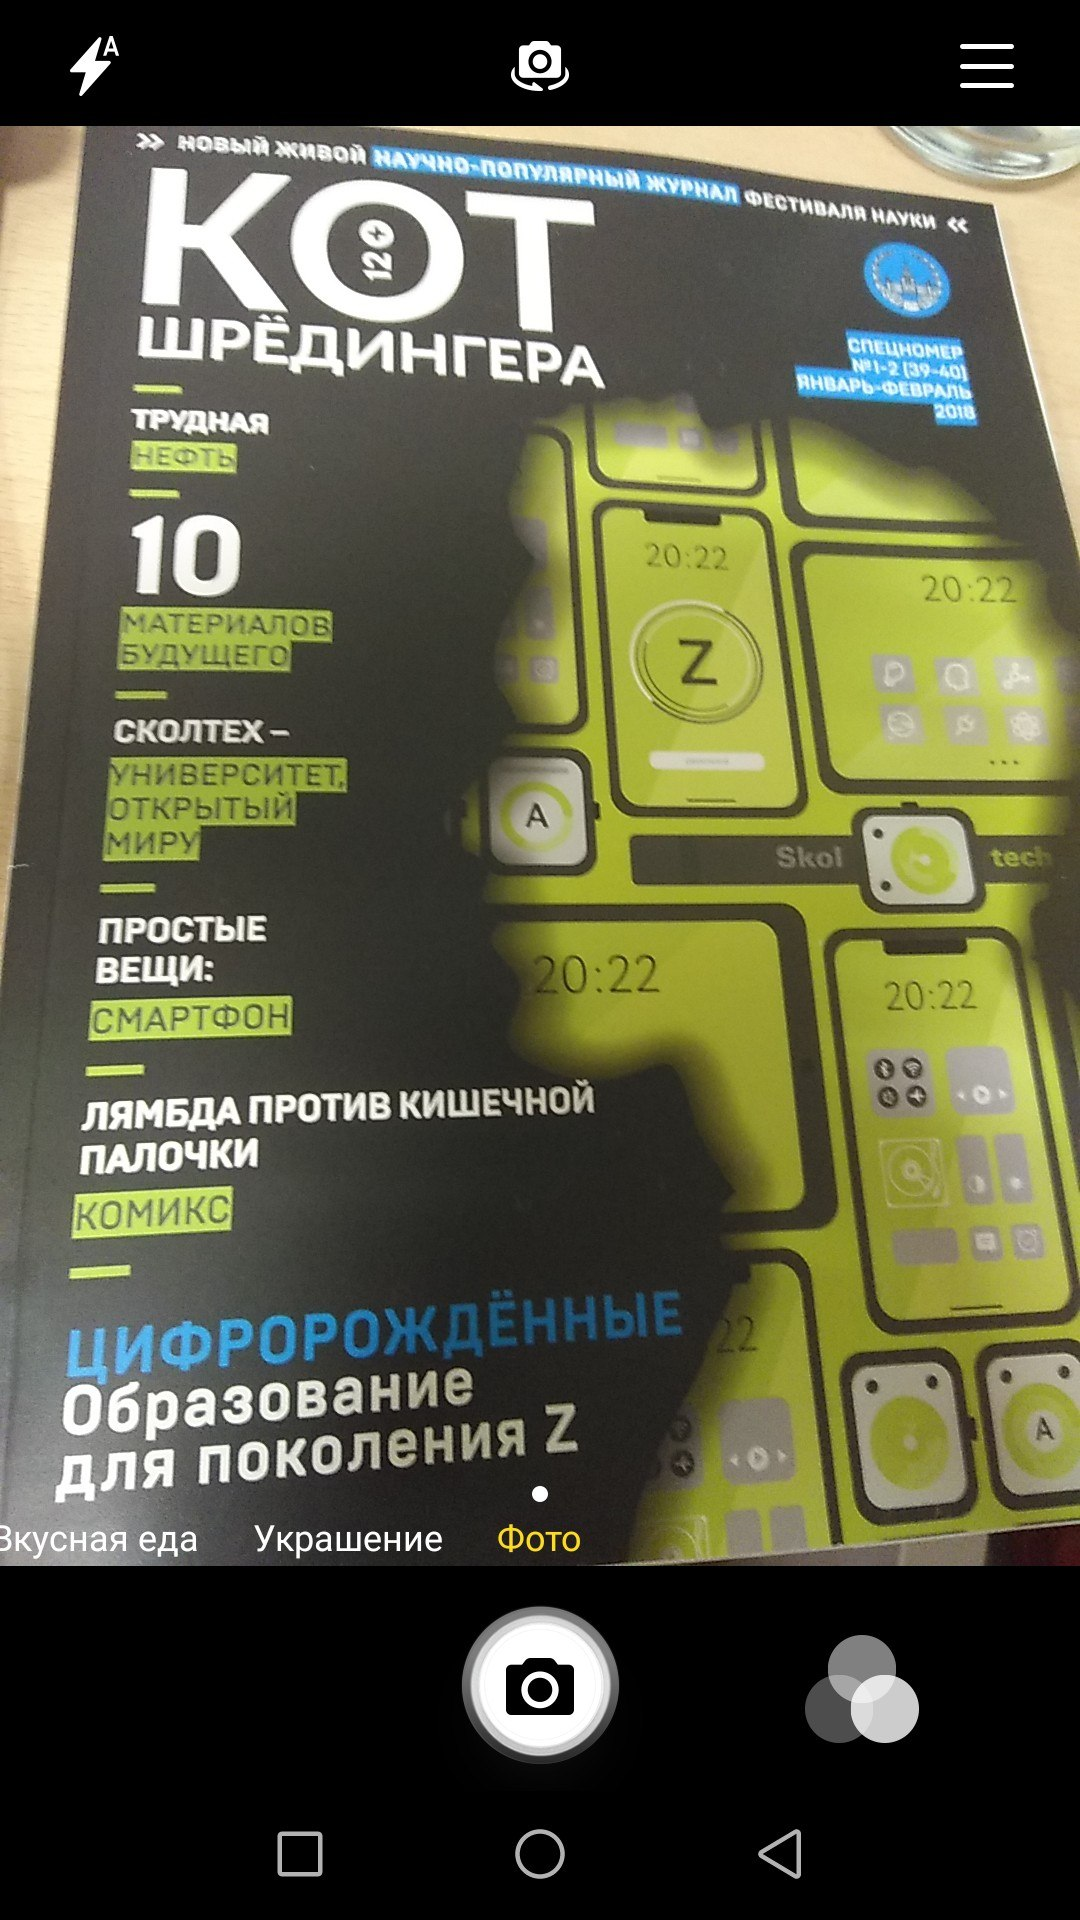
\includegraphics[width=0.4\linewidth]{pics/main}
	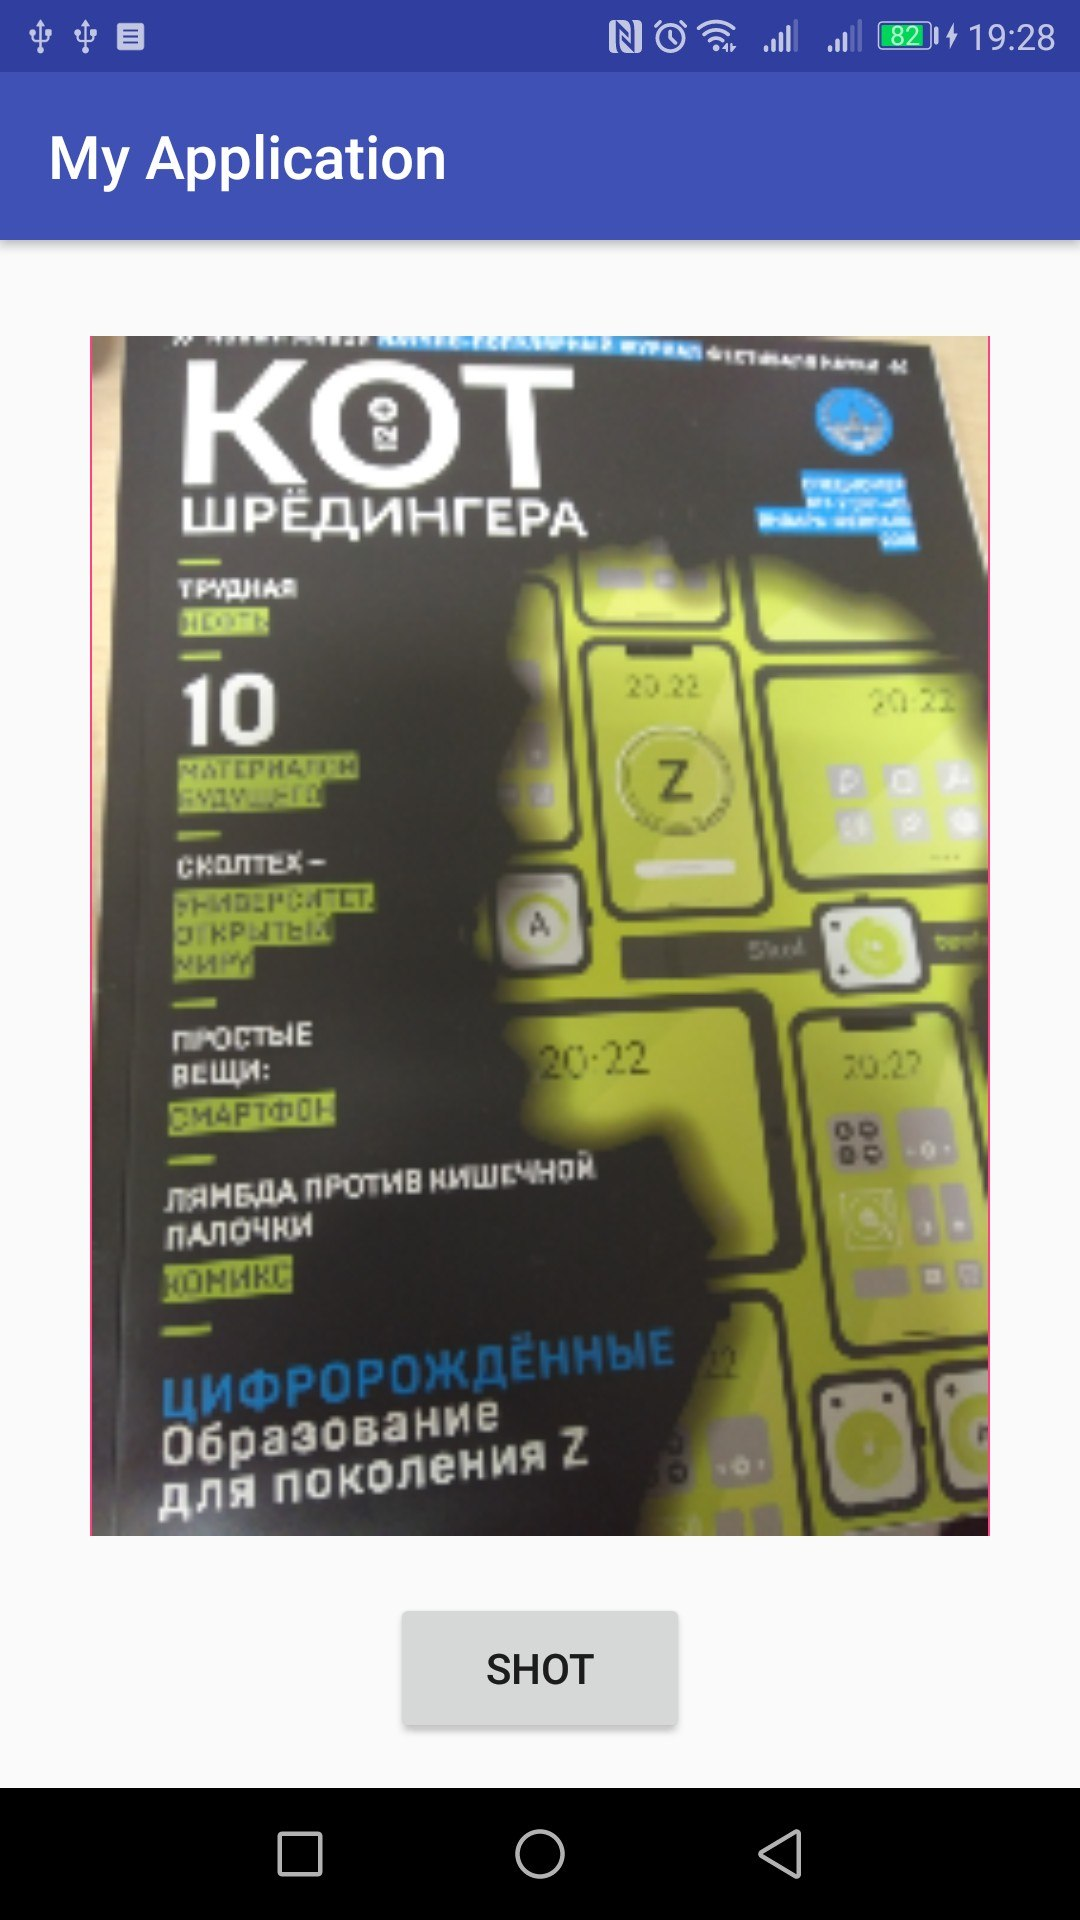
\includegraphics[width=0.4\linewidth]{pics/camera}
	\caption{Результат работы приложения}
	\label{fig:my}
\end{figure}